\documentclass{article}
\usepackage[T1]{fontenc}
\usepackage[utf8]{inputenc}
\usepackage[hidelinks]{hyperref}  
\newcommand{\click}[2]{\href{http://#1}{\colorlet{temp}{.}\color{blue}{\underline{\color{temp}#2}}\color{temp}}} 
\usepackage{fixltx2e}
\usepackage{amssymb}
\usepackage{amsmath}
\usepackage[dvipsnames]{xcolor}
\usepackage{soul}


\colorlet{yelloww}{green!10!orange!90!}
\usepackage[margin=.8in]{geometry}
\usepackage[authordate,bibencoding=auto,strict,backend=biber,natbib]{biblatex-chicago}

\usepackage{qtree}

\usepackage{graphicx}
\graphicspath{ {./images/} }

%\usepackage{xcolor}
%\usepackage{pagecolor}
%\usepackage{lipsum}  

\usepackage{tgadventor}

%\pagecolor{black}
%\color{white}

\addbibresource{./bibliography.bib}

\title{Learning Structured Representation for Text Classification via Reinforcement Learning}
\author{Blogpost by Lisa Becker (775242) }
\date{May 2020}

\begin{document}

\maketitle

\section{TL;DR}
Text classification used to either ignore sentence structure or used one which has been either manually annotated by humans or learned under human supervision. \cite{zhang2018} developed and tested two neural nets which learn Structured Representation of sentences with Reinforcement Learning for a sentiment text classification task:
\begin{itemize}
    \item \textbf{Information Distilled Long Short-Term Memory (ID-LSTM)} removes task-irrelevant words.
    \item \textbf{Hierarchically Structured Long Short-Term Memory (HS-LSTM)} builds phrases, similar to a two-level syntax tree \href{https://www.youtube.com/watch?v=69iB-xy0u4A}{( - syntax shrubbery?)}
\end{itemize}
These two algorithms outperformed other methods without Reinforcement Learning in three out of four corpora.
\section{Introduction}
In this blogpost, I first want to introduce you to the authors in this same paragraph, then convince you about the importance of
\begin{itemize}
    \item \nameref{sec:strucrep}, and introduce you to
    \item \nameref{sec:rlmodel}, consisting of
    \begin{enumerate}
        \item \textbf{\nameref{sec:pnet}},
        \item \textbf{\nameref{sec:models}} and
        \item \textbf{\nameref{sec:cnet}}
    \end{enumerate}
    \item \nameref{sec:training}
    \item \nameref{sec:data},
    \item \nameref{sec:testing}, and lastly
    \item \nameref{sec:cents}
\end{itemize}

\begin{figure}[!h]
    \centering

\includegraphics[scale=.35]{catthrow.png}
    \label{fig:my_label}
    \caption{May I lure you into reading with cats or nerdy memes?}
\end{figure}
\newpage

The authors of the paper are Tianyang Zhang, \href{http://coai.cs.tsinghua.edu.cn/hml/}{Minlie Huang} (both associated with the Tsinghua University) and \href{https://www.microsoft.com/en-us/research/people/lizo/}{Li Zhao} (former PhD student of said University, now working for Microsoft). Their paper got presented at and published by the \href{https://www.aaai.org/ocs/index.php/AAAI/AAAI18/paper/view/16537/16174}{AAAI Conference on Artificial Intelligence} in 2018 and is also available at \href{https://www.microsoft.com/en-us/research/wp-content/uploads/2017/11/zhang.pdf}{Microsoft}. But let's dive right into (a very short) history of text representation and classification:\\\\
The earlier methods used for text representation can be roughly divided into four types: \par
\begin{enumerate}
    \item \textbf{Word bag representation models:}  Deep Average Network Autoencoders. The main problem with this approach is that the word order is ignored.
    \item \textbf{Sequence representation models:} Convolutional Neural Networks (CNN) and Recurrent Neural Networks (RNN) consider the word order, but without using any sentence structure.
    \item \textbf{Structural representation models:} Tree-structured Long Short-Term Memory (LSTM), recursive autoencoders. Although considering sentence structure, a structured representation needs to be constructed with the help of a pre-specified parse-tree.
    \item \textbf{Attention-based models:} Use the attention mechanism to differentially score input words or sentences to build representations. (\href{https://www.youtube.com/watch?v=SysgYptB198}{If you want to have a look at Attention models, let it be better explained by yours truly than by me, *click*.})
\end{enumerate}

\cite{zhang2018} thought they could do better - and they did. Let me show you how - but before I have to explain to you why structured language is important and why we want algorithms to find their own structures.

\section{The Importance of Structured Representation}\label{sec:strucrep}
In the four kinds of models named above, the structure of language was either provided by a human annotator or predicted with human supervision. But so far there aren't many convincing models which construct a structured representation of language without human intervention.\\\\ But why is structured representation so important and how is it connected to language?\\

\begin{figure}[h]
    \centering
    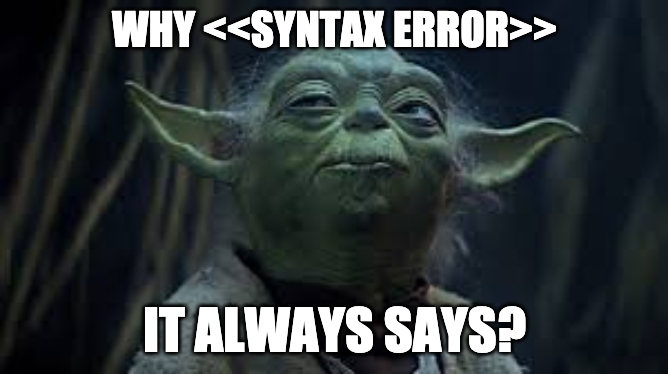
\includegraphics[scale=.4]{syntaxerror.png}
    \caption[Not only programming languages need syntax. Human languages need syntax too!]{Not only programming languages need syntax. Human languages need syntax too!}
    \label{fig:yoda}
\end{figure}
\newpage

If you know Yoda\footnote{Yoda was just too perfect of an example not to be used to draw your attention to syntax. In case you're neither a fan or cats nor the Star Trek nor the Star Wars Franchise, I apologise for the pain and bad jokes that you're going through.} from the Star Wars Franchise, you probably noticed he has speaks in a funny way: it's because he uses a different syntax than Standard English!\footnote{\href{https://slate.com/technology/2019/12/baby-yoda-first-words-linguistics.html}{Don't we all wonder whether Baby Yoda will speak the same way? *click*}}. That is, because \textbf{language isn't simply a linear sequence of words}. As we notice when we get a <<syntax error>> while writing code or listen to Yoda, there's a set of rules and exceptions in each language that describes in what order and under which restrictions we're allowed to place words (or functions, arguments, variables...)\footnote{\href{https://www.youtube.com/watch?v=n9168PgGHBc}{*Click* here if you'd like to dig a bit deeper into the basics of English syntax, phrases and binding constraints.}}. As a human, we can make sense of Yoda's speech because he actually makes use of syntax, just not the one of Standard English. We can even make sense of sentences that appear to be in a complete arbitrary word order by applying semantics and world knowledge. But it's a different story for a computer: Without structure, we get <<syntax errors>>. \\\\  
Now that we know that \textbf{language has underlying structures, how do we make a computer understand them?} If you look at older machine learning algorithms you'll see that they rely on the input being a feature and then learn a classifier, regressor, etc. on top of that. Most of these features (=structures) were handcrafted, meaning, they were designed by humans. This means that we would give the rules that we are assuming about English syntax to the algorithm so it uses them to either process or produce language. The problem here is that they were designed by humans which means that they are based on heuristics. It is \textbf{our} representation of language - biased, because it is made by humans for humans. This is were Knowledge Representation comes in.\\\\
\textbf{Knowledge Representation} is a part of Artificial Intelligence and simply means that we \textbf{try to encode real-life (or human) knowledge in a way that a computer understands it and can use it to solve complex problems} (\href{http://www.deeplearningbook.org/contents/representation.html}{*click here* to dive in deeper)}. Language structure is an excellent example of a representation of human knowledge that a computer can use to comprehend and produce sentences. Up to now, researchers have given the computer the exact rules on how to put words together to comprehend or produce sentences. But what if the machine could figure out the structure by itself? Reinforcement Learning (RL) builds its own strategies to solve a problem by trial and error. \href{https://www.wired.com/2016/03/two-moves-alphago-lee-sedol-redefined-future/}{This way, an RL agent can even develop solutions that are new to humans *click*}.
\\\\ The two models proposed by the \cite{zhang2018} are supposed to build sentence representations in that manner: figuring out structures of language by themselves and then use it to classify texts. To achieve that, the \textbf{ID-LSTM is supposed to rely on "task-relevant words"}, so it deletes words of its input that are not necessary for classification. \textbf{HS-LSTM on the other hand discovers "task-relevant phrase structures" and builds sentence representations with two-levels}.
\newpage

\section{The Reinforcement Learning Model}\label{sec:rlmodel}
The two models proposed by the authors consists of each three parts:
\begin{enumerate}
    \item \textcolor{BlueViolet}{the Policy Network (PNet)},
    \item \textcolor{Maroon}{the two Structured Representation Models: ID-LSTM and HS-LSTM} and
    \item \textcolor{yelloww}{the Classification Network (CNet)},
\end{enumerate}

The algorithm traverses through a sentence (X = x\textsubscript{1}, x\textsubscript{2}, ... x\textsubscript{L}), looking at one word at a time(step t). At each word x\textsubscript{t}, the \textcolor{Maroon}{\textbf{structured representation model ID-LSTM or HS-LSTM}} calculates the state s\textsubscript{t} and hands it back to the \textcolor{BlueViolet}{\textbf{PNet}}. The \textcolor{BlueViolet}{\textbf{PNet}} takes the state s\textsubscript{t} and decides with its policy and parameters $\Theta$ which action a\textsubscript{t} to take next. After the action is chosen, \textcolor{BlueViolet}{\textbf{PNet}} feeds it to the \textcolor{Maroon}{\textbf{structured representation model}}. This way, the \textcolor{BlueViolet}{\textbf{PNet}} and the \textcolor{Maroon}{\textbf{structured representation model}} play "ping pong" (or rather, "state action") until the end of the sentence is reached. Lastly, the \textcolor{BlueViolet}{\textbf{PNet}} and \textcolor{Maroon}{\textbf{structured representation model}}, proud parents of a sentence representation in form of a hidden state h, hand their newborn to the \textcolor{yelloww}{\textbf{CNet}}. The \textcolor{yelloww}{\textbf{CNet}} classifies this text representation into one of the possible categories (or class labels), compares, whether this matches with the actual category (/label), calculates a reward and gives this delayed reward back to the \textcolor{BlueViolet}{\textbf{PNet}}. The \textcolor{BlueViolet}{\textbf{PNet}} takes this feedback into account and adjusts its parameters accordingly, such that the next sentence representation leads to an even more accurate classification. We'll dive a bit deeper into the three components in the next paragraphs.


\begin{figure}[h]
    \centering
    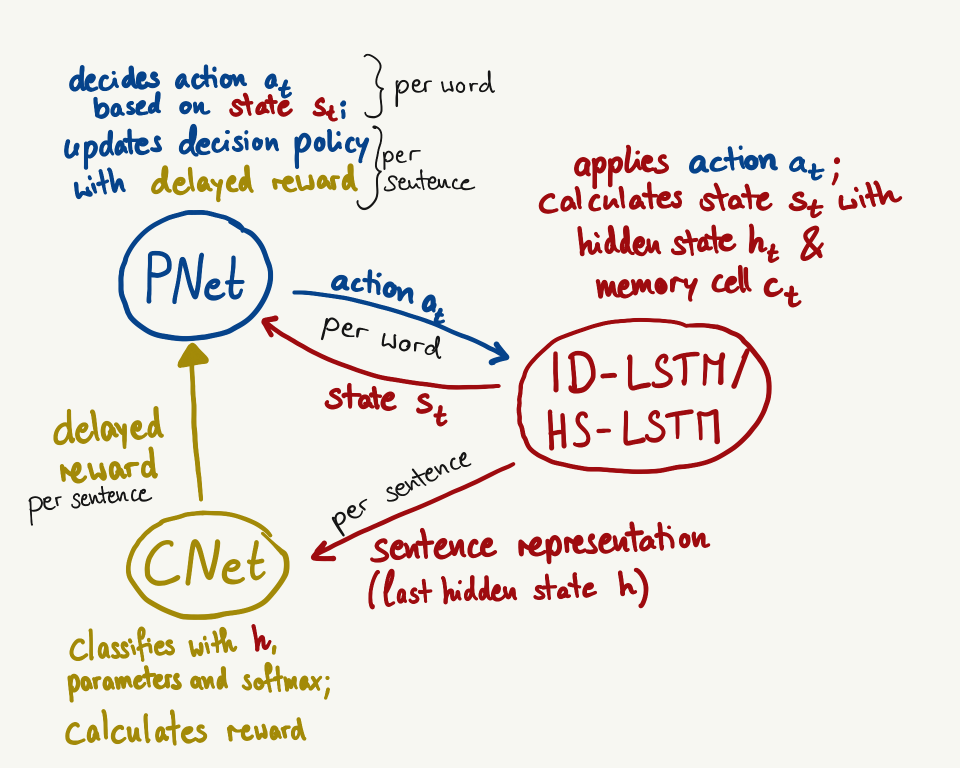
\includegraphics[scale=.4]{alg_overview.png}
    \caption{Overview of the algorithm.}
\end{figure}

\subsection{\textcolor{BlueViolet}{The Policy Network (PNet)}}\label{sec:pnet}
Formally, the \textcolor{BlueViolet}{\textbf{PNet}} looks like this: $\pi(a_t|s_t;\Theta) = \sigma(W * s_t +b)$. The parameters $\Theta $ (which consist of the weight W and the bias b), are optimised by the REINFORCE\footnote{I don't mean to shout at you just to make clear that we're talking about Reinforcement learning, but REINFORCE is actually an acronym for \textbf{RE}ward \textbf{I}ncrement = \textbf{N}onnegative \textbf{F}actor
x \textbf{O}ffset Reinforcement x \textbf{C}haracteristic \textbf{E}ligibility} algorithm, as Johann described last week, and policy gradient methods to maximise the expected reward. 
Many other Reinforcement Learning agents, which make use of the deterministic \href{https://becominghuman.ai/lets-build-an-atari-ai-part-0-intro-to-rl-9b2c5336e0ec?gi=d08d6f863052}{Q-Learning (*click*)}, allow no exploration in their policy but it has to be handled separately. It also makes it difficult to handle continuous actions: Since we traverse through the input word by word, the current decision (action) affects the following decisions, but the reward is only received much later after the completion of the sentence. Thus, Q-Learning is very inefficient for the task of language processing! The policy gradient method, as the name suggests, allows a gradient movement within the policy to determine the optimal parameters, adjusted after each sentence. \cite{sutton2000}

\subsection{\textcolor{Maroon}{The two Structured Representation Models: ID-LSTM and HS-LSTM}} \label{sec:models}
An overview of the two algorithms can be seen in Figure \ref{fig:lstms_overview}.\\\\
The \textcolor{Maroon}{\textbf{ID-LSTM}} "distills" the input and removes words and phrases that are not relevant to the task, such as determiners, conjunctions or even whole phrases like "than it first sets out to be": So it decides for each word whether to \{retain\} or \{delete\} it. Formally, for each word x in a sentence X = x\textsubscript{1}, x\textsubscript{2} ,... x\textsubscript{L}, the \textcolor{BlueViolet}{\textbf{PNet}} tells us to either \{retain\} or \{delete\} it by providing us with a parallel structure of actions A = a\textsubscript{1}, a\textsubscript{2},... a\textsubscript{L}. While the algorithm traverses through the input, at each word x, it calculates a state s. The state s\textsubscript{t} is determined through a vector concatenation of the memory cell c\textsubscript{t-1}, the hidden state h\textsubscript{t-1} and the current word x\textsubscript{t}. The state s\textsubscript{t} gets fed back into the \textcolor{BlueViolet}{\textbf{PNet}} which gives us a new action a\textsubscript{t} based on its policy and so forth. If the model decides to \textbf{delete} a word x, the memory cell and hidden state from the last retained word get copied to calculate the state of the next time step t. If the model decides to \textbf{retain} a word x, the memory cell and hidden state calculate a new memory call and hidden state "with all gate functions and the update function" which are not further described. The authors found that the \textcolor{Maroon}{\textbf{ID-LSTM}} mainly left words of sentiment and negation, which looks regarding the task!\\\\
Similar to ID-LSTM, the \textcolor{Maroon}{\textbf{HS-LSTM}} model calculates a state s, action a, memory cell c and hidden state h for each word x while we're traversing through the sentence. At each word x\textsubscript{t}, the \textcolor{BlueViolet}{\textbf{PNet}} decides with the state s\textsubscript{t} from the \textcolor{Maroon}{\textbf{representation model}} whether the word x\textsubscript{t} is \{inside\} a phrase or at the \{end\} of a phrase and gives that decision back to the \textcolor{Maroon}{\textbf{representation model}} in form of an action\textsubscript{t}. This happens on two levels: on a word and on a phrase level. If an action\textsubscript{t} indicates that word x\textsubscript{t} is at the \{end\} of a phrase in the word-level LSTM, the hidden state h\textsubscript{t} is handed to the phrase-level LSTM. If the action a\textsubscript{t} indicates that the word x\textsubscript{t} is inside a phrase, the hidden state of the previous position t is copied to the phrase-level LSTM. Similar like the ID-LSTM copies h and c from the previous word, when the action indicates to delete a word! So the behaviour of \textcolor{Maroon}{\textbf{HS-LSTM}} both relies on the action on the current position t and the previous position t-1:\\
\begin{table}[h]
    \centering
    \begin{tabular}{cc|c}
        Previous action & Current action & Behaviour\\
         a\textsubscript{t-1} & a\textsubscript{t} & of Phrase \\
         \hline
        Inside & Inside & Phrase continues \\
        Inside & End & Phrase ends \\
        End & Inside & Phrase begins \\
        End & End & Phrase consists of one word \\
    \end{tabular}
    \caption{Overview over the action combinations and their meaning.}
\end{table}

\begin{figure}[h]
    \centering
    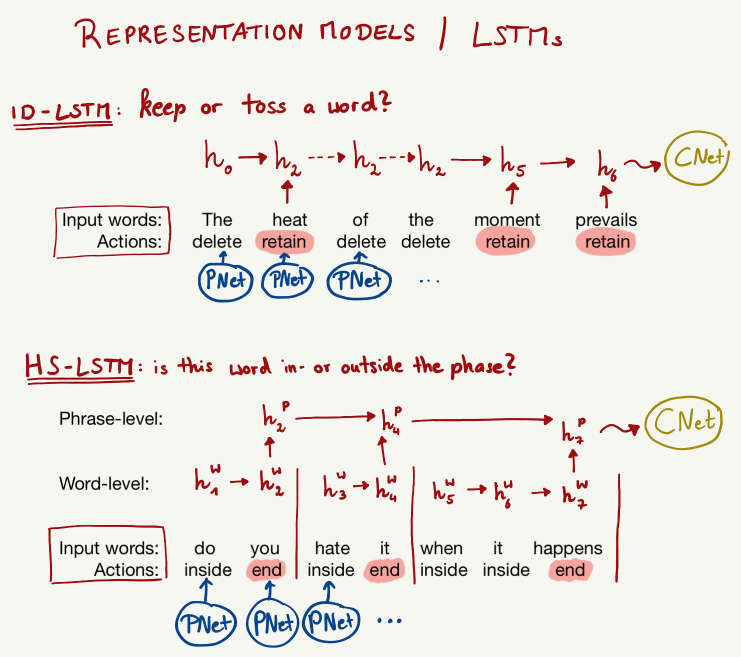
\includegraphics[scale=.4]{lstms_overview.png}
    \caption{The basic idea of \textcolor{Maroon}{\textbf{ID-LSTM}} and \textcolor{Maroon}{\textbf{HS-LSTM}}.}
    \label{fig:lstms_overview}

\end{figure}
\newpage

\subsection{\textcolor{yelloww}{The Classification Network (CNet)}}\label{sec:cnet}
The probability distribution over the sentence representation and the class labels is calculated as follows:\\\\
\textcolor{Maroon}{\textbf{ID-LSTM}}: P(\textit{y}|X) = \textit{softmax}(W\textsubscript{s}h$_L$ + b\textsubscript{s})\\
\textcolor{Maroon}{\textbf{HS-LSTM}}: P(\textit{y}|X) = \textit{softmax}(W\textsubscript{s}h$^p_L$ + b\textsubscript{s})\\\\
Where P(\textit{y}|X) denotes how likely it is that sample X is classified as y. W and b are the weight and bias factors which aren't further explained in the paper, h is the hidden state that we get from the \textcolor{Maroon}{\textbf{representation model}} (\textcolor{Maroon}{\textbf{ID-LSTM}} or \textcolor{Maroon}{\textbf{HS-LSTM}}). The softmax function from the classifier ensures that we always have at least some non-zero value in the hidden state vectors. The superscript P in the \textcolor{Maroon}{\textbf{HS-LSTM}} describes that the hidden state h comes from the phrase level representation. Subscript L denotes that the hidden state h is from the last word of the sentence.  \\\\
Since \textcolor{Maroon}{\textbf{ID-LSTM}} and \textcolor{Maroon}{\textbf{HS-LSTM}} are doing two different things (removing words or building phrases), the reward R is calculated differently. I spare you the math on this one, but this is roughly how the \textcolor{yelloww}{\textbf{CNet}} calculates the reward R for \textcolor{Maroon}{\textbf{ID-LSTM}} and \textcolor{Maroon}{\textbf{HS-LSTM}} are the following:\\\\
\textcolor{Maroon}{\textbf{ID-LSTM}}: Remove as many words as possible! $\rightarrow$ higher reward with fewer words\\
\textcolor{Maroon}{\textbf{HS-LSTM}}: A good phrase structure has neither too many nor too few phrases! $\rightarrow$ higher reward with 3-4 phrases per 10 words

\section{Training}\label{sec:training}
All three parts, \textcolor{BlueViolet}{\textbf{PNet}}, \textcolor{Maroon}{\textbf{representation Models ID-LSTM / HS-LSTM}} and \textcolor{yelloww}{\textbf{CNet}} are trained at the same time, because they depend on another. Without diving to deep into the maths, here's the training process in a nutshell:
\begin{enumerate}
    \item Pre-training of \textcolor{Maroon}{\textbf{ID-LSTM}} and \textcolor{Maroon}{\textbf{HS-LSTM}}, and \textcolor{yelloww}{\textbf{CNet}} with cross-entropy as loss function.
    \begin{enumerate}
        \item \textcolor{Maroon}{\textbf{ID-LSTM}}: original sentence without deletion is used for pre-training.
        \item \textcolor{Maroon}{\textbf{HS-LSTM}}: sentence is split in predefined phrases.
    \end{enumerate}
    \item Pre-train \textcolor{BlueViolet}{\textbf{PNET}} with the parameters of the \textcolor{Maroon}{\textbf{ID-LSTM}} / \textcolor{Maroon}{\textbf{HS-LSTM}}.
    \item Train all three parts together until convergence.
    
\end{enumerate}
\begin{figure}[h]
    \centering

\includegraphics[scale=.4]{data.png}
    \label{fig:my_label}
    \caption{Who could say no to Captain Picard?}
\end{figure}

\section{"It's Data, not Data"} \label{sec:data}
\cite{zhang2018} didn't use only one, but four different corpora for their testing:
\begin{enumerate}
    \item \href{http://www.cs.cornell.edu/people/pabo/movie-review-data/}{\textbf{MR}, "Polarity dataset": a movie review sentiment analysis dataset with positive/negative reviews \citep{pang-lee-2005}}
    \item \href{https://nlp.stanford.edu/sentiment/index.html}{\textbf{SST}, "Stanford Sentiment Treebank", a movie review sentiment analysis dataset with a 1-5 rating scale (Socher et al. 2013)\footnote{\href{https://nlp.stanford.edu/sentiment/index.html}{I recommend the comment section on the datasets website in case you want to be entertained by and lost in discussions for a while.}}}
    \item \href{http://www.cs.cornell.edu/people/pabo/movie-review-data/}{\textbf{Subj}, "Subjectivity dataset": a movie review sentiment analysis dataset with subjective and objective "reviews" (= plot summaries in the objective class) \citep{pang-lee-2004}}
    \item \href{http://nlpprogress.com/english/text_classification.html}{\textbf{AG}, "AG News corpus": a large topic classification dataset constructed by Zhang, Zhao, LeCun 2015. The topics are sports, world, business and sci/tech}
\end{enumerate}
... four different datasets! That seems like pretty solid, broad testing. But... is it really?\par
In case you enthusiastically clicked already on all four datasets to have a closer look, you might have noticed that MR and Subj share the same href. Why is that? - Because the datasets come from the same source. In \cite{zhang2018}'s paper and on the website of the corpora, it's not even clear which paper from Pang and Lee refers to which corpus, so I had to dig in the original papers, which dataset referred to which paper on the source homepage. Both concern movie reviews which were either classified on a 1-5 rating scale or into "subjective" and "objective" reviews. The former only investigates subjective reviews, while the latter classifies whether a movie review is subjective or just a summary of the plot. SST is also a movie review dataset and if you have a closer look, it is actually based on the MR dataset. The only dataset diverging from the topic is the AG corpus, which is a subset of a bigger corpus and contains 30.000 training and 1.900 testing samples, divided into four classes. All four datasets, although from the early 2000's, are very popular and still widely used in computational linguistics with several thousand citations each, according to Google Scholar - which might be the reason why the authors didn't explain them any further or even gave reason why they used them: it's because they're so widely known (- and now they are to me too)!

\begin{figure}[h]
    \centering

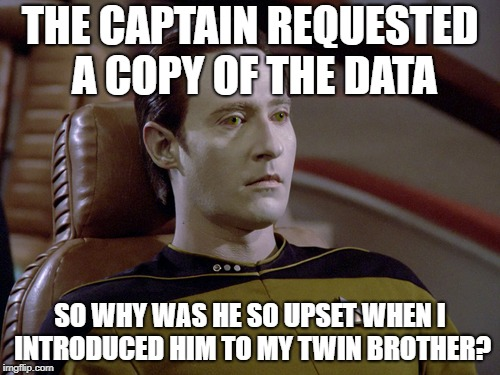
\includegraphics[scale=.5]{datatwin.jpg}
    \label{fig:my_label}
\end{figure}

\section{Putting it to the test} \label{sec:testing}
 For good research, you want to compare your new model to something else when testing on the data to see whether your model is actually contributing (and in which form). The \textbf{baselines} that were used to evaluate \textcolor{Maroon}{\textbf{ID-LSTM}} and \textcolor{Maroon}{\textbf{HS-LSTM}} can be divided into three categories:
\begin{enumerate}

    \item \textbf{Basic neural models:} a sequencential LSTM from \cite{tai-etal-2015}, a biLSTM which is commonly used in text classification (here, the authors don't even bother to mention which/whose implementation they're using) and a CNN from \cite{kim-2014}.
    \item \textbf{Models relying on re-specified parsing structure:} RAE (Recursive Auto Encoder) from \cite{socher-etal-2011} and a Tree-LSTM \citep{tai-etal-2015} which both rely on a predefined parsing structure.
    \item \textbf{Models distilling important information by attention mechanism:} a structured Self-Attentive model, which uses an attention mechanism and regularisation term to construct sentence embeddings \citep{lin2017}
\end{enumerate} \par

Table \ref{tab:results} shows that the \textcolor{Maroon}{\textbf{HS-LSTM model}} achieved the highest accuracy in three of four corpora. Only in the SST corpus it was outperformed by the Tree-LSTM model by .3\%.\\ So, the authors managed to build a Reinforcement Learning agent that outperforms the other models with the \textcolor{Maroon}{\textbf{HS-LSTM performing}} slightly better than the \textcolor{Maroon}{\textbf{ID-LSTM}}! Sounds like something - at least in combination with those datasets and baselines.

\begin{table}[h]
    \centering
    \begin{tabular}{ll|cccc}
    \hline
         & Models & MR & SST & Subj & AG  \\
         \hline
         1. &LSTM & 77.4* & 46.4* & 92.2 & 90.9 \\
            &biLSTM & 79.7* & 49.1* & 92.8 & 91.6 \\
            &CNN & 81.5* & 48.0* & 93.4* & 91.6 \\
         \hline
         2. &RAE & 76.2* & 47.8 & 92.8 & 90.3 \\
            &Tree-LSTM & 80.7* & \textbf{50.1} & 93.2 & 91.8 \\
         \hline
        3.  &Self-Attentive & 80.1 & 47.2 & 92.5 & 91.1\\
        \hline
            &ID-LSTM & 81.6 & 50.0 & 93.5 & 92.2 \\
            &HS-LSTM & \textbf{82.1} & 49.8 & \textbf{93.7} & \textbf{92.5}\\
        \hline
         
    \end{tabular}
    \caption{Classification accuracy in \% on different datasets with different methods. Bold indicates the best performance per dataset, asterix indicates classification results from other papers.}
    \label{tab:results}
\end{table}

\cite{zhang2018} also performed a qualitative and quantitative analysis of both their models. In a nutshell, the \textcolor{Maroon}{\textbf{ID-LSTM}} removed words with little "sentiment" which interestingly (but not surprisingly) overlap roughly with the words of highest frequency described by Zipf's Law (\textit{the} 84.40\%, \textit{by} 86.96\%, \textit{of} 99.18\% ...). Some words were also words that were never deleted (\textit{not}, \textit{no}, \textit{good}, \textit{interesting}). The word \textit{but} was only removed in 7.81\% of its appearances.\par

\begin{table}[h]
    \centering
    \begin{tabular}{l|ccccc}

        
            \hline
         Average in words & MR & SST & Subj & AG\\
         \hline
        Sentence length     & 21.25 & 19.16 & 24.73 & 35.12\\
         Shortened length   & 11.57 & 11.71 & 9.17 & 13.05\\
        Amount of deleted words & 9.68 & 7.45 & 15.56 & 22.07\\
        
        \hline

    \end{tabular}
    \caption{\textcolor{Maroon}{\textbf{ID-LSTM}} qualitative analysis. }
    \label{tab:id-lstm}
\end{table}

According to \cite{zhang2018} \textcolor{Maroon}{\textbf{HS-LSTM}} sometimes fails to find the "correct" boundary between phrases, but instead builds "longer and more complete phrases". They base that assumption on the comparison to their predefined sentence structures:

\begin{table}[h]
    \centering
    \begin{tabular}{l|l}

    
         \hline
        Original text & Much smarter and more attentive than it first sets out to be .\\
        ID-LSTM & Much smarter \st{and more} attentive \st{than it first sets out to be} .\\
        HS-LSTM & Much smarter | and more attentive | than it first sets out to be .\\
        \hline

    \end{tabular}
    \caption{Example of a sentence representation by each \textcolor{Maroon}{\textbf{models}}.}
    \label{tab:id-lstm}
\end{table}

\section{My two cents} \label{sec:cents}
Personally, I would've preferred to have a deeper look into the qualitative analysis of the \textcolor{Maroon}{\textbf{HS-LSTM model}}. As a trained general theoretical linguist, my heart beat a bit higher while reading about the idea of a model that learns building some sort of syntactic hierarchy by itself. \textcolor{Maroon}{\textbf{HS-LSTM}} seems to produce phrases which are more flexible in length and content than "traditional" phrases according to human-designed syntax. RL agents which discover syntactical rules on their own might be a possibility for us humans to learn structures about language that we haven't come across yet or even to make us rethink how we've looked at language structure so far. A linguist may dream.
\begin{figure}[h]
    \centering


\includegraphics[scale=.3]{picardsmile.png}
    \label{fig:my_label}
    \caption{*okay, technically it would only give evidence to a highly-debated, decades-old theory that only a handful of people still support. Not, that general theoretical linguistics would get much attention (let alone funding) these days.}
\end{figure}

Next to this paper giving me unrealistic daydreams and lots\footnote{Some might say "too many".} of ideas for Star Trek memes, there were \textbf{a few things that I liked less about it}:\begin{itemize}
    \item their choice of \textbf{baselines}: with artificial intelligence and deep learning as some of the fastest growing fields, I highly doubt that the chosen baselines are still state-of-the-art given the fact that the corresponding papers were published between 2011 and 2017 (but, to be fair, said paper was published in 2018). It was never claimed by the authors that the baselines are state-of-the-art, but I wonder whether there are other algorithms out there that outperform \textcolor{Maroon}{\textbf{ID-LSTM}} and \textcolor{Maroon}{\textbf{HS-LSTM}} on these or other datasets. Further, I can't imagine that \textcolor{Maroon}{\textbf{ID-LSTM}} and \textcolor{Maroon}{\textbf{HS-LSTM}} are the first algorithm of their kind (i.e., an LSTM that builds syntax). In the introduction, they mention that \cite{yogatama2016} built a binary tree structure for sentence representation and that \cite{chung2017} also already proposed a hierarchical representation model. Why didn't they attempt to compare to these approaches? Further, the researchers who put the SST Stanford Sentiment Treebank corpus together already achieved a classification accuracy of >80\%, while and \cite{zhang2018} only achieved around 50\%, as did all the other baselines \citep{socher-etal-2011}.
    \item their choice of \textbf{datasets}: I find it a bit dubious that they barely described their datasets and made it so hard to figure out which corpora they exactly used. Maybe I would've known about them if I wasn't completely new to Reinforcement Learning and sentiment analysis, so more information about the corpora would be redundant to researchers in the field. But I still don't know why they used exactly these corpora except for the fact that they're popular (yet pretty old) corpora for sentiment classification. It's curious that they have three corpora with movie reviews and one with news articles. Not exactly the same domain?
    \item their choice of \textbf{training}: instead of training the algorithm from scratch, they used predefined structures for pre-training. Here I'm sceptical about the \textcolor{Maroon}{\textbf{HS-LSTM}}. They feed it phrases that they split themselves "and also use some simple heuristics". I wonder how big of an influence the human-split phrases have on the training process of the algorithm and what kind of heuristics that are. I'd like to see what happens if they trained the algorithm from scratch: would \textcolor{Maroon}{\textbf{HS-LSTM}} build different kinds of phrases?
\end{itemize}

Following my complaints, I suggest the following for \textbf{future research}: 
\begin{itemize}
    \item testing the method on other domains than sentiment analysis text classification (that's what the authors suggest as well).
    \item within the topic of sentiment analysis, test the method on other corpora (and choose appropriate baselines).
    \item trying to train the \textcolor{Maroon}{\textbf{HS-LSTM}} from scratch and give it different kinds of input for pre-training in order to compare the differently trained \textcolor{Maroon}{\textbf{HS-LSTM models}}.
    \item try to incorporate more levels on the \textcolor{Maroon}{\textbf{HS-LSTM}}: would it build syntax trees similar to the ones that we suggest?
\end{itemize}

I hope you enjoyed reading this blogpost despite my attempts of funniness and learned something new. Last but not least: wash your hands, don't lick doorhandles, stay safe and take care. - Hold on! I've got a last one for you:

\begin{figure}[h]
    \centering

\includegraphics[scale=.4]{doors.png}
\end{figure}
\printbibliography
\end{document}
 